\documentclass{article}[18pt]
\usepackage{/home/sam/Documents/School_Notes/format}
\lhead{AS Level Physics - Electricity}

\begin{document}
\begin{center}
\underline{\huge Current electricity}
\end{center}
\section{Basics of electricity}
\begin{itemize}
\item Current - The rate of flow of charge
\item Potential difference - Work done per unit charge
\end{itemize}
\section{Current-voltage characteristics}
\subsection{Ohmic Conductor}
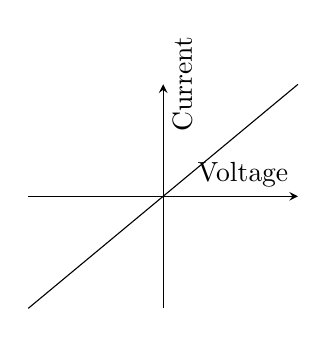
\begin{tikzpicture}
\begin{axis}[axis lines=middle, ticks=none,scale=0.5,    ylabel = Current,xlabel=Voltage,ylabel style={rotate=90}
]
\addplot[color=black]{x};
\end{axis}
\end{tikzpicture}
\subsection{Bulb}
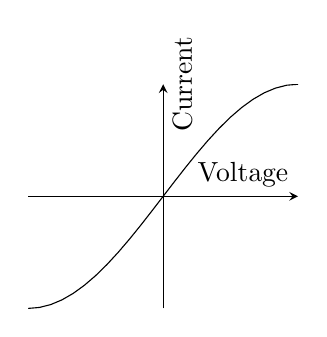
\begin{tikzpicture}
\begin{axis}[axis lines=middle, ticks=none,scale=0.5,    ylabel = Current,xlabel=Voltage,ylabel style={rotate=90}
]
\addplot[color=black,domain=-90:90]{sin(x)};
\end{axis}
\end{tikzpicture}
\subsection{Diode}
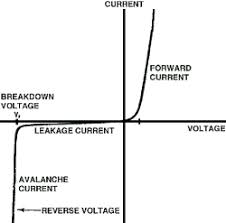
\includegraphics[width=2in]{diode.jpeg}\\
Ohm's Law: Current is proportional to voltage\\
\newpage
\section{Resistivity}
$\downarrow$ Temperature $\downarrow$ Resistance of any conductor\\
\\
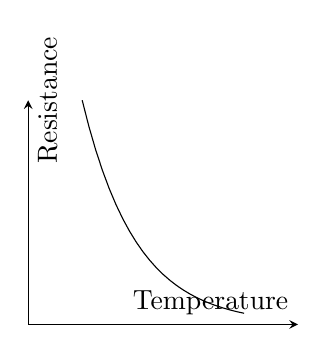
\begin{tikzpicture}
\begin{axis}[axis lines=middle, ticks=none,scale=0.5,    ylabel = Resistance,xlabel=Temperature,ylabel style={rotate=90},xmin=0,xmax=5,ymin=0
]
\addplot[color=black,domain=1:4]{1/exp(x)};
\end{axis}
\end{tikzpicture}
\section{Superconductivity}
Below a certain temperature (critical temperature) the resistance of a material will be zero, this is described as superconductivity. The critical temperature depends on the material.\\
\\
Applications:\\
\begin{itemize}
\item Producing strong magnetic fields
\item The reduction in energy loss when transmitting power
\end{itemize}
\section{Circuits}
\subsection{Resistors}
\textbf{Series}: $R_T=R_1+R_2+R_3...$\\
\\
\textbf{Parallel}: $\dfrac{1}{R_T}=\dfrac{1}{R_1}+\dfrac{1}{R_2}+\dfrac{1}{R_3}...$
\subsection{Current}
\textbf{Series}: Current in = Current out. Current through multiple components is the same as through one\\
\textbf{Parallel}: Current into a junction = current out of a junction
\subsection{Voltage}
\textbf{Series}: Total voltage = the sum of voltages in the circuit\\
\textbf{Parallel}: Voltage in parallel components is equal
\section{Potential Dividers}
A potential divider is used to supply constant or variable potential difference from a power supply\\
\\
$\mathlarger{V_{Out}=V_{In}\dfrac{R_1}{R_1+R_2}}$\\
\\
Potential dividers can be used as part of sensor circuits to increase or decrease voltage based on environmental conditions\\
\newpage
\section{Electromotive force and internal resistance}
\begin{tabularx}{\textwidth}{|X|X|}
\hline
Switch Open&Switch Closed\\
\hline
Voltmeter reads $\epsilon$&Voltmeter reads $\epsilon-IR$\\
\hline
\end{tabularx}
\subsection{Voltage Current Graph}
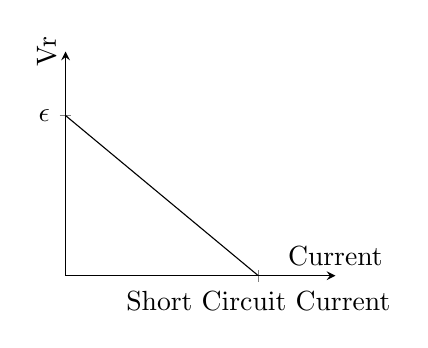
\begin{tikzpicture}
\begin{axis}[axis lines=middle,scale=0.5,    ylabel = Vr,xlabel=Current,ylabel style={rotate=90,anchor=south},xlabel style={anchor=south},xmin=0,xmax=7,ymin=0,ymax=7,xtick={5},xticklabels={Short Circuit Current},ytick={5},yticklabels={$\epsilon$}
]
\addplot[color=black,domain=0:5]{-x+5};
\end{axis}
\end{tikzpicture}

\end{document}
